% Компіляція: lualatex -shell-escape main.tex (двічі)
\documentclass[12pt,a4paper]{article}

\usepackage{fontspec}
\usepackage{polyglossia}
\setdefaultlanguage{ukrainian}
\setmainfont{NewComputerModern10}
\setsansfont{Noto Sans}
\setmonofont{Noto Sans Mono}[
  Scale=0.82,
  ItalicFont={Noto Sans Mono},
  ItalicFeatures={FakeSlant=0.2}
]

\usepackage{
  amsmath,
  amssymb,
  array,
  booktabs,
  caption,
  enumitem,
  float,
  geometry,
  graphicx,
  microtype,
  titlesec,
  xcolor
}
\geometry{left=2cm,right=2cm,top=2cm,bottom=2cm}
\setlength{\parindent}{1.25cm}
\setlength{\parskip}{0pt}
\linespread{1.08}

\titleformat{\section}
  {\normalfont\fontsize{14}{16}\selectfont\bfseries}
  {\thesection}{0.6em}{}
\titleformat{\subsection}
  {\normalfont\fontsize{12}{14}\selectfont\bfseries}
  {\thesubsection}{0.6em}{}
\titlespacing*{\section}{0pt}{1.4em}{0.65em}
\titlespacing*{\subsection}{0pt}{1.1em}{0.45em}
\captionsetup{font=small,labelfont=bf,labelsep=endash}
\captionsetup[table]{position=bottom,skip=5pt}

\usepackage[newfloat]{minted}
\SetupFloatingEnvironment{listing}{name=Лістинг}
\setminted{
  fontsize=\scriptsize,
  linenos,
  breaklines,
  breakanywhere,
  frame=single,
  framesep=2mm,
  bgcolor=gray!5,
  tabsize=4
}

\usepackage[
  unicode,
  colorlinks=true,
  linkcolor=black,
  urlcolor=blue,
  pdftitle={ІО-41, Давидчук А. М., Паралельні та розподілені обчислення, Лабораторна робота №2.1},
  pdfauthor={Давидчук Артем Миколайович},
  pdfsubject={Синхронізація потоків. Варіант 17}
]{hyperref}

\newcommand{\studentName}{Давидчук А. М.}
\newcommand{\studentGroup}{ІО-41}
\newcommand{\recordBook}{4106}
\newcommand{\teacherName}{Корочкін О. В.}
\newcommand{\reportYear}{2026}

\usepackage{tikz}
\usetikzlibrary{arrows.meta,shapes.geometric,positioning,calc,fit}
\usepackage{longtable}
\usepackage{needspace}
\begin{document}

\pagenumbering{gobble}
\begin{titlepage}
  \begin{center}
    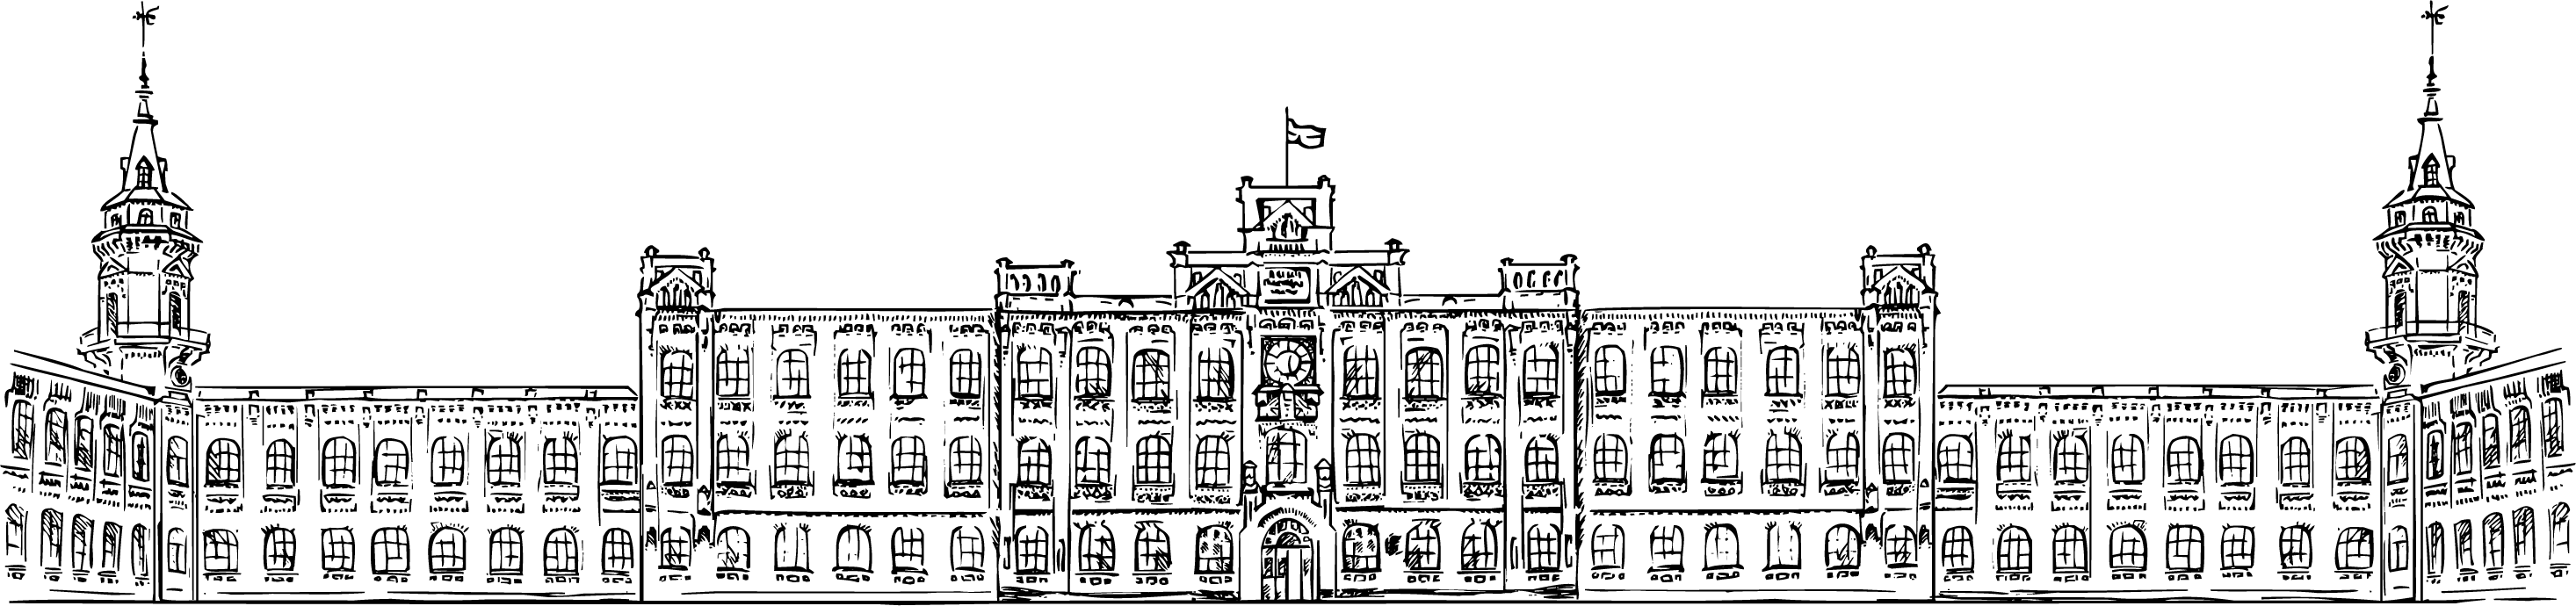
\includegraphics[width=0.7\textwidth]{../../../../../../templates/letterhead.png}
  \end{center}

  \begin{center}
    \large
    Національний технічний університет України\\
    «Київський політехнічний інститут імені Ігоря Сікорського»\\[1em]
    Факультет інформатики та обчислювальної техніки\\
    Кафедра обчислювальної техніки
  \end{center}

  \vfill

  \begin{center}
    \textbf{\LARGE Паралельні та розподілені обчислення}\\[2em]
    \textbf{\Large Лабораторна робота №2.1}\\[0.7em]
    \parbox{0.9\textwidth}{\centering
      «Програмування для систем зі спільною пам’яттю.\\ Засоби синхронізації PThread»}
  \end{center}

  \vfill

  \begin{flushright}
    \begin{minipage}{0.48\textwidth}
      Виконав: студент 3 курсу ФІОТ,\\
      групи \studentGroup\\
      \textit{\studentName}\\
      Залікова книжка № \recordBook\\
      Варіант завдання: 17\\[1em]
      Перевірив: \textit{\teacherName}
    \end{minipage}
  \end{flushright}

  \vfill

  \begin{center}Київ --- \reportYear\end{center}
\end{titlepage}

\pagenumbering{arabic}

\section{Тема та мета роботи}

\noindent\textbf{Тема:} програмування для комп’ютерних систем зі спільною
пам’яттю з використанням семафорів, м’ютексів, критичних секцій,
атомарних змінних і бар’єрів.

\medskip
\noindent\textbf{Мета:} розробити паралельний алгоритм обчислення
векторно-матричного виразу; організувати взаємодію чотирьох потоків мовою C
засобами POSIX Threads і C11; забезпечити взаємне виключення під час
введення та виведення, синхронізацію етапів і правильне об’єднання
проміжних результатів; дослідити завантаження процесора та прискорення.

\section{Завдання}

За варіантом 17 таблиці завдань до ЛР2--ЛР4 потрібно обчислити
\begin{equation}
 E=(B\cdot MR)\cdot(MM\cdot MO)+\min(B)\cdot Q\cdot d.
 \label{eq:task}
\end{equation}
Тут $B,Q,E$ --- вектори довжини $N$; $MR,MM,MO$ --- квадратні матриці
порядку $N$; $d$ --- скаляр. Вектори у добутках із матрицями
розглядаються як вектори-рядки. Кількість потоків $P=4$.
Розподіл введення та виведення наведено в табл.~\ref{tab:io}.

\begin{table}[H]
\centering\renewcommand{\arraystretch}{1.2}
\begin{tabular}{|c|c|c|}\hline
\textbf{Потік} & \textbf{Введення} & \textbf{Виведення}\\\hline
$T_1$ & $MR,Q$ & $E$\\\hline
$T_2$ & $B,MM$ & ---\\\hline
$T_3$ & $MO,d$ & ---\\\hline
$T_4$ & --- & ---\\\hline
\end{tabular}
\caption{Розподіл операцій введення та виведення для варіанта 17}
\label{tab:io}
\end{table}

Виконання роботи включає розроблення паралельного математичного
алгоритму, виявлення спільних ресурсів, опис алгоритмів усіх потоків із
критичними ділянками та точками синхронізації, структурну схему взаємодії,
реалізацію програми і тестування на одному та чотирьох ядрах.

\section{Опис програми}

\subsection{Структура програми}

Програму написано мовою C стандарту C11. Проєкт складається з
\texttt{main.c}, модуля \texttt{include/data.h},
\texttt{include/data.c} та файла \texttt{CMakeLists.txt}.
Головний модуль створює чотири потоки з функціями \texttt{F1}--\texttt{F4},
передаючи всім адресу однієї структури \texttt{shared\_memory}.
Модуль \texttt{Data} містить типи векторів і матриць, операції виділення
та звільнення пам’яті, заповнення й допоміжні математичні функції.

Елементи зберігаються в динамічних масивах типу \texttt{long long}.
Матриці розміщено по рядках: елемент $(i,j)$ має індекс
\texttt{(size\_t)i * N + j}. Пам’ять для всіх вхідних, проміжних і
результуючих масивів виділяється до створення потоків.

У поточній реалізації перевіряється додатність $N$. Для кожного вхідного
вектора або матриці вводиться одне ціле число заповнення; скаляр $d$
вводиться окремо. Додаткових фіксованих меж введення немає. Запрошення та читання даних одного
потоку виконуються в одній критичній секції. Послідовність отримання
м’ютекса потоками $T_1,T_2,T_3$ не фіксується, але їхні діалоги не
перемішуються. Потік $T_4$ нічого не вводить, проте бере участь у всіх
обчислювальних етапах.

\subsection{Паралельний математичний алгоритм}

Уведемо проміжні результати:
\begin{equation}
 V=B\cdot MR,\qquad MX=MM\cdot MO,\qquad m=\min(B).
\end{equation}
Тоді кінцевий вираз набуває вигляду $E=V\cdot MX+mQd$.

Для потоку з номером $t\in\{0,1,2,3\}$ визначимо
\begin{equation}
 a_t=\left\lfloor\frac{tN}{4}\right\rfloor,\qquad
 b_t=\left\lfloor\frac{(t+1)N}{4}\right\rfloor,\qquad
 J_t=\{a_t,\ldots,b_t-1\}.
 \label{eq:ranges}
\end{equation}
Потік $T_{t+1}$ записує лише елементи й стовпці з індексами $j\in J_t$.
Діапазони покривають усі індекси без перетинів, зокрема коли $N$ не
кратне чотирьом. Якщо діапазон порожній, обчислювальні цикли
пропускаються, але потік усе одно проходить бар’єри та сигналізує про
завершення.

Перший обчислювальний етап складається з таких операцій:
\begin{align}
 V_j &= \sum_{k=0}^{N-1}B_k MR_{k,j}, && j\in J_t,\\
 MX_{i,j} &= \sum_{k=0}^{N-1}MM_{i,k}MO_{k,j},
 && i=0,\ldots,N-1,\quad j\in J_t,\\
 m_t &= \min_{j\in J_t}B_j,\qquad
 m=\min(m_0,m_1,m_2,m_3).
\end{align}
Для порожнього $J_t$ у програмі використовується нейтральне значення
\texttt{LLONG\_MAX}. Часткові мінімуми об’єднуються атомарним
зменшенням спільної змінної \texttt{min\_b}.

Після синхронізації потоків на бар’єрі проміжних результатів кожен
потік обчислює свою частину кінцевого вектора:
\begin{equation}
 E_j=\sum_{k=0}^{N-1}V_k MX_{k,j}+mQ_jd,\qquad j\in J_t.
 \label{eq:result}
\end{equation}
Для одного $E_j$ потрібен увесь готовий $V$, тому очікування завершення
першого етапу є обов’язковим. Власні стовпці $MX$ потік уже обчислив сам.

Основне навантаження становить множення матриць: загальна складність
$O(N^3)$, приблизно $N^3/4$ ітерацій внутрішнього циклу на потік.
Пам’ять для чотирьох матриць і чотирьох векторів за 8-байтових елементів
становить $32N^2+32N$ байт без урахування службових структур.

\subsection{Спільні ресурси та засоби синхронізації}

Спільна структура містить $N,B,Q,E,MR,MM,MO,d,V,MX$.
М’ютекс, бар’єри, семафор, атомарний мінімум і позначки часу оголошено
глобально. Локальними є межі діапазону, індекси циклів, суми та
частковий мінімум кожного потоку.

\begin{table}[H]
\centering\small\renewcommand{\arraystretch}{1.2}
\begin{tabular}{|p{1cm}|p{4.1cm}|p{9.3cm}|}\hline
\textbf{Знак} & \textbf{Об’єкт програми} & \textbf{Призначення}\\\hline
$M_1$ & \texttt{console\_mutex} & Взаємне виключення для консолі; захищає критичні ділянки введення $CS_{\rm in}$ і друку $CS_{\rm out}$.\\\hline
$A_1$ & \texttt{min\_b} & Атомарний мінімум. Початкове значення \texttt{LLONG\_MAX}; оновлення через compare-exchange.\\\hline
$B_1$ & \texttt{input\_ready} & Бар’єр на 4 учасники. Два проходи: завершення введення та публікація початкового часу.\\\hline
$B_2$ & \texttt{intermediate\_ready} & Бар’єр на 4 учасники після запису $V$, $MX$ та оновлення мінімуму.\\\hline
$S_1$ & \texttt{finished} & Один семафор, початковий лічильник 0. По одному сигналу від $T_2,T_3,T_4$ та три очікування в $T_1$.\\\hline
\end{tabular}
\caption{Позначення об’єктів на структурній схемі}
\label{tab:sync}
\end{table}

Вхідні дані не змінюються після $B_1$. Потоки записують неперетинні
ділянки $V,MX,E$, тому м’ютекс навколо обчислень не потрібний.
Бар’єри відділяють запис від подальшого спільного читання.
Атомарне порівняння із заміною не дозволяє перезаписати менший мінімум
більшим. М’ютекс консолі завжди звільняється до очікування на бар’єрі.

\subsection{Алгоритми потоків}

За позначеннями методичних прикладів $S_{j,k}$ означає сигнал задачі
$T_j$, а $W_{j,k}$ --- очікування події в задачі $T_j$; $k$ є номером
взаємодії цієї пари задач. Для завершення обчислень кожна пара
взаємодіє один раз, тому $k=1$. На схемі $T_2,T_3,T_4$ мають точки
$S_{1,1}$. Логічним залежностям $W_{2,1},W_{3,1},W_{4,1}$
відповідає один вузол $T_1$: три очікування спільного семафора.
У коді ці очікування реалізовано трьома викликами \texttt{sem\_wait}
одного семафора без прив’язки порядку сигналів до конкретного потоку.

\subsubsection*{Потік $T_1$ (функція F1)}
\begin{enumerate}[leftmargin=*,itemsep=0.15em]
\item У критичній ділянці під $M_1$ ввести $MR,Q$; звільнити м’ютекс.
\item Пройти $B_1$ двічі; визначити $J_0$.
\item Обчислити $V_{J_0}$, стовпці $MX_{:,J_0}$ та локальний мінімум $B_{J_0}$.
\item Атомарно зменшити $A_1$; пройти $B_2$.
\item Прочитати остаточний мінімум і обчислити $E_{J_0}$.
\item Дочекатися завершення $T_2,T_3,T_4$: $W_{2,1},W_{3,1},W_{4,1}$.
\item Зафіксувати кінцевий час. У критичній ділянці під $M_1$ вивести весь $E$.
\item Звільнити м’ютекс і завершити потік.
\end{enumerate}

\Needspace{12\baselineskip}
\subsubsection*{Потік $T_2$ (функція F2)}
\begin{enumerate}[leftmargin=*,itemsep=0.15em]
\item У критичній ділянці під $M_1$ ввести $MM,B$; звільнити м’ютекс.
\item Пройти $B_1$ двічі; визначити $J_1$.
\item Обчислити $V_{J_1}$, стовпці $MX_{:,J_1}$ та локальний мінімум $B_{J_1}$.
\item Атомарно зменшити $A_1$; пройти $B_2$.
\item Обчислити $E_{J_1}$; подати сигнал $S_{1,1}$ через $S_1$ і завершити потік.
\end{enumerate}

\subsubsection*{Потік $T_3$ (функція F3)}
\begin{enumerate}[leftmargin=*,itemsep=0.15em]
\item У критичній ділянці під $M_1$ ввести $MO,d$; звільнити м’ютекс.
\item Пройти $B_1$ двічі; визначити $J_2$.
\item Обчислити $V_{J_2}$, стовпці $MX_{:,J_2}$ та локальний мінімум $B_{J_2}$.
\item Атомарно зменшити $A_1$; пройти $B_2$.
\item Обчислити $E_{J_2}$; подати сигнал $S_{1,1}$ через $S_1$ і завершити потік.
\end{enumerate}

\subsubsection*{Потік $T_4$ (функція F4)}
\begin{enumerate}[leftmargin=*,itemsep=0.15em]
\item Без введення перейти до двох проходів $B_1$; визначити $J_3$.
\item Обчислити $V_{J_3}$, стовпці $MX_{:,J_3}$ та локальний мінімум $B_{J_3}$.
\item Атомарно зменшити $A_1$; пройти $B_2$.
\item Обчислити $E_{J_3}$; подати сигнал $S_{1,1}$ через $S_1$ і завершити потік.
\end{enumerate}

\clearpage
\subsection{Структурна схема взаємодії потоків}

Схему на рис.~\ref{fig:structure} побудовано за додатком В методички
(с.~14) і принципом рис.~6.2 прикладів. Вона показує спільні ресурси,
засоби взаємного виключення та зв’язок сигналів із відповідними
очікуваннями. Нижня частина окремо показує бар’єри тих самих потоків:
спочатку $B_1$, обчислення проміжних даних, $B_2$, обчислення $E$,
і лише потім сигнали завершення, показані у верхній частині.

\begin{figure}[H]
\centering
% Структурна схема: позначення за додатком В методички.
\begin{tikzpicture}[x=1cm,y=1cm,>=Stealth,font=\small,
 task/.style={draw,thick,trapezium,trapezium left angle=80,
 trapezium right angle=100,fill=yellow!13,align=center},
 resource/.style={draw,ellipse,fill=green!9,align=center,font=\scriptsize},
 port/.style={draw,ellipse,fill=yellow!25,minimum width=1.25cm,minimum height=.48cm,font=\scriptsize},
 wait/.style={port,fill=red!12},
 barrier/.style={draw,thick,fill=gray!7,align=center},
 access/.style={dashed,gray!75,thin}]
\draw[thick] (-.2,-9.05) rectangle (15.6,1.05);
\node[fill=white] at (7.7,1.05) {\textbf{Спільна пам’ять і засоби взаємодії}};
\node[resource,minimum width=3.1cm] (io) at (2.4,.3) {Консоль: $M_1$ ($T_1$--$T_3$)\\$CS_{\rm in},\ CS_{\rm out}$};
\node[resource,minimum width=3.1cm] (atom) at (7.65,.3) {$A_1$: \texttt{min\_b}\\атомарне зменшення: $T_1$--$T_4$};
\node[resource,minimum width=3.5cm] (data) at (12.9,.3) {$B,Q,MR,MM,MO,d$\\$V,MX,E$};
\draw[access] (io.south) -- (2.4,-.5) -- (12.9,-.5) -- (data.south);
\draw[access] (atom.south) -- (7.65,-.5);
\draw[thick,fill=yellow!13] (.7,-1.05) -- (3.7,-1.05) -- (3.0,-5.2) -- (0,-5.2) -- cycle;
\coordinate (t1top) at (2.25,-1.05);
\node[align=center] at (1.7,-2.2) {\textbf{$T_1$}\\$MR,Q\to E$};
\node[font=\scriptsize,align=center] at (1.7,-4.5) {$J_0$\\виведення $E$};
\foreach \n/\yy/\inp/\jj in {2/-1.7/{$B,MM$}/1,3/-3.15/{$MO,d$}/2,4/-4.6/{без введення}/3}{
 \draw[thick,fill=yellow!13] (11.65,{\yy+.48}) -- (14.4,{\yy+.48}) -- (14.2,{\yy-.48}) -- (11.45,{\yy-.48}) -- cycle;
 \node[align=center] at (12.95,\yy) {\textbf{$T_\n$}\quad $J_\jj$\\\inp};
 \coordinate (t\n-left) at (11.55,\yy);
 \coordinate (t\n-right) at (14.3,\yy);
 \node[port] (s\n) at (10.55,\yy) {$S_{1,1}$};
 \draw[->] (t\n-left) -- (s\n.east);
}
\draw[access] (2.4,-.5) -- (t1top);
\draw[access] (14.9,-.5) -- (14.9,-4.6);
\draw[access] (12.9,-.5) -- (14.9,-.5);
\foreach \n in {2,3,4} {\draw[access] (t\n-right) -- (14.9,0 |- t\n-right);}
\node[draw,thick,fill=blue!5,minimum width=2.6cm,minimum height=4.3cm,align=center] (sem) at (7.7,-3.15) {$S_1$\\\texttt{finished}\\лічильник\\початково 0};
\foreach \n/\yy in {2/-1.7,3/-3.15,4/-4.6}{
 \draw[->] (s\n.west) -- (sem.east |- s\n.west);
}
\node[draw,rounded corners,fill=red!12,align=center,font=\scriptsize,
 minimum width=2.2cm,minimum height=1.1cm] (waitall) at (4.95,-3.15)
 {$T_1$: $3\times$ \texttt{sem\_wait}\\без визначення\\відправника};
\draw[->] (sem.west) -- (waitall.east);
\draw[->] (waitall.west) -- (3.346,-3.15);
\node[font=\scriptsize] at (7.7,-5.65) {Сигнали надходять після запису відповідних частин $E$};
\draw[gray!50] (.2,-5.95) -- (15.2,-5.95);
\node[font=\small] at (7.7,-6.2) {Окремий вигляд: бар’єри тих самих потоків (до сигналів вище)};
\foreach \i/\xx in {1/1.9,2/5.75,3/9.6,4/13.45}{
 \node[draw,minimum width=1.3cm,minimum height=.42cm] (b\i) at (\xx,-6.72) {$T_\i$};
 \draw[->] (b\i.south) -- (\xx,-7.25);
}
\node[barrier,minimum width=14.9cm,minimum height=.5cm] at (7.7,-7.5) {$B_1$: введення завершено; повторний прохід після запису \texttt{start\_time}};
\foreach \xx in {1.9,5.75,9.6,13.45} {\draw[->] (\xx,-7.75) -- (\xx,-8.27);}
\node[fill=white,font=\scriptsize] at (7.7,-8.0) {обчислення $V$, $MX$ та $m$};
\node[barrier,minimum width=14.9cm,minimum height=.5cm] at (7.7,-8.52) {$B_2$: усі проміжні результати готові; далі кожен потік обчислює $E_{J_t}$};
\end{tikzpicture}

\caption{Структурна схема взаємодії потоків для варіанта 17}
\label{fig:structure}
\end{figure}

\noindent\textbf{Позначення:} $M$ --- м’ютекс; $CS$ --- критична секція;
$A$ --- атомарна змінна; $B$ --- бар’єр; $S$ --- семафор.
Суцільні стрілки у верхній частині показують передачу сигналів
завершення; штрихові зв’язки --- доступ до спільних ресурсів.

Усі три сигнали надходять до одного $S_1$, а не до трьох різних
семафорів. Кожен потік $T_2$--$T_4$ сигналізує рівно один раз.
Окремого об’єкта події \texttt{Event} у поточній реалізації немає:
готовність етапів забезпечують $B_1,B_2$, завершення обчислень --- $S_1$.

\subsection{Створення потоків і вимірювання часу}

Головний потік перевіряє введення $N$, виділення пам’яті та
ініціалізацію засобів синхронізації, після чого запускає
\texttt{F1}--\texttt{F4} через \texttt{pthread\_create}.
Помилка створення будь-якого потоку завершує процес до очікування
\texttt{join}, щоб уже запущені потоки не чекали відсутнього учасника
бар’єра нескінченно. Після всіх \texttt{pthread\_join} знищуються
семафор, бар’єри, м’ютекс і звільняються масиви.

Вимірювання виконується через \texttt{CLOCK\_MONOTONIC}.
Після першого проходу $B_1$ один потік із кодом повернення
\texttt{PTHREAD\_BARRIER\_SERIAL\_THREAD} записує початковий час.
Повторний прохід того самого бар’єра не дозволяє почати обчислення
раніше за цей запис. Потік $T_1$ фіксує кінцевий час після отримання
трьох сигналів, але до друку $E$:
\begin{equation}
 t=(s_2-s_1)+\frac{ns_2-ns_1}{10^9}.
\end{equation}
Отже, інтервал охоплює обчислення, планування та синхронізацію,
але не введення, створення потоків і виведення результату.

Введення виконується через \texttt{scanf} з перевіркою кількості
успішно прочитаних значень. Недодатне $N$, нечислове введення та кінець
вводу завершують процес повідомленням про помилку. Очікування семафора
повторюється при \texttt{EINTR}.

Тип \texttt{long long} розширює діапазон результатів, але не забезпечує
арифметику необмеженої точності. Вхідні дані слід обирати так, щоб усі
добутки та суми вміщувалися в цей тип; автоматичного контролю
арифметичного переповнення поточна програма не виконує.

\section{Тестування та результати}

\subsection{Перевірка правильності обчислень}

Якщо всі елементи вхідних даних і скаляр $d$ дорівнюють одному числу $c$,
то $V_j=Nc^2$, $MX_{i,j}=Nc^2$, $\min(B)=c$. Для кожного елемента
результату отримуємо
\begin{equation}
 E_j=N^3c^4+c^3.
\end{equation}

\begin{table}[H]
\centering\renewcommand{\arraystretch}{1.15}
\begin{tabular}{|r|r|r|c|}\hline
$N$ & $c$ & Очікуване $E_j$ & Перевірка\\\hline
1 & 1 & 2 & збігається\\\hline
3 & 1 & 28 & збігається\\\hline
4 & 1 & 65 & збігається\\\hline
5 & 2 & 2008 & збігається\\\hline
8 & $-2$ & 8184 & збігається\\\hline
100 & 9 & 6561000729 & збігається\\\hline
1000 & 1 & 1000000001 & збігається\\\hline
1200 & 1 & 1728000001 & збігається\\\hline
\end{tabular}
\caption{Контрольні результати для сталого заповнення даних}
\end{table}

При $N=4$, $c=1$ програма виводить:
\begin{minted}[fontsize=\footnotesize]{text}
Completed. E result:
[65, 65, 65, 65]
\end{minted}

Розміри $N=1,3,5$ перевіряють порожні або нерівні діапазони;
від’ємне $c$ --- коректність мінімуму. Випадок $N=100,c=9$ дає результат
поза діапазоном 32-бітного \texttt{int}, але коректний для
\texttt{long long}. На тестовій копії також використано неоднорідні
знакові дані для $N=1,3,5,8$; отримані значення порівняно з незалежним
послідовним обчисленням $((BMR)MM)MO+\min(B)Qd$ і виявлено збіг.
Некоректні $N=0,-1$, нечислові значення та кінець вводу завершують
процес повідомленням про помилку. Після спрощення введення додатково
перевірено $N=2$, $c=101$: отримано правильне $E_j=833513509$.

\subsection{Дослідження часу виконання}

Контрольні запуски проведено 12.10.2026 у Linux на AMD Ryzen 7 7730U:
8 фізичних ядер і 16 логічних CPU. Використано GCC 16.2.1,
параметри \texttt{-std=c11 -O0 -pthread}. Для $N=1000$ та $N=1200$
всі вхідні дані й $d$ заповнено одиницями; у кожному режимі виконано
три запуски з чергуванням режимів. Значення часу взято з виводу самої
програми; усі елементи результату перевірено за формулою $N^3+1$.
Числа збережено у \texttt{measurements.json}. Ці вимірювання виконано
до спрощення допоміжних функцій введення та перевірок; математичний
алгоритм і межі вимірювання часу залишилися такими самими. Для оновленої
редакції коду окремі вимірювання продуктивності не проводилися.

Обмеження CPU виконується командою \texttt{taskset}. Запуск із каталогу
\texttt{src}:
\begin{minted}[fontsize=\footnotesize]{bash}
cmake -S . -B build
cmake --build build
taskset -c 0 ./build/lab2
taskset -c 0,2,4,6 ./build/lab2
\end{minted}

За даними \texttt{lscpu -e=CPU,CORE,SOCKET}, CPU 0 і 1 належать
одному фізичному ядру, CPU 2 і 3 --- наступному тощо.
Тому набір $0,2,4,6$ використовує чотири різні фізичні ядра.
В обох режимах програма створює чотири потоки; на одному CPU вони
ділять процесорний час. \texttt{taskset} задає дозволений набір CPU,
але не закріплює кожен потік за окремим ядром.

\begin{table}[H]\centering\renewcommand{\arraystretch}{1.2}
\begin{tabular}{|c|c|c|}\hline Номер запуску & Одне ядро, с & Чотири ядра, с\\\hline
1 & $2{,}285847$ & $0{,}602125$\\\hline
2 & $2{,}305389$ & $0{,}646983$\\\hline
3 & $2{,}308227$ & $0{,}624484$\\\hline
Середнє & $2{,}299821$ & $0{,}624531$\\\hline\end{tabular}
\caption{Час виконання для $N=1000$}
\end{table}
Для $N=1000$ коефіцієнт прискорення та ефективність становлять
\begin{equation} K_p=\frac{t_1}{t_4}=\frac{2{,}299821}{0{,}624531}=3{,}682,\qquad \eta=\frac{K_p}{4}\cdot100\%\approx 92{,}1\%.\end{equation}
\begin{table}[H]\centering\renewcommand{\arraystretch}{1.2}
\begin{tabular}{|c|c|c|}\hline Номер запуску & Одне ядро, с & Чотири ядра, с\\\hline
1 & $3{,}978902$ & $1{,}107869$\\\hline
2 & $3{,}987936$ & $1{,}158707$\\\hline
3 & $4{,}066953$ & $1{,}132493$\\\hline
Середнє & $4{,}011264$ & $1{,}133023$\\\hline\end{tabular}
\caption{Час виконання для $N=1200$}
\end{table}
Для $N=1200$ коефіцієнт прискорення та ефективність становлять
\begin{equation} K_p=\frac{t_1}{t_4}=\frac{4{,}011264}{1{,}133023}=3{,}540,\qquad \eta=\frac{K_p}{4}\cdot100\%\approx 88{,}5\%.\end{equation}
Величина $t_1$ є часом тієї самої чотирипотокової програми на одному
CPU, а не часом іншої послідовної реалізації. Результати залежать від
оптимізації компілятора, частоти, кешів і фонового навантаження.
Додаткові запуски на CPU 0--3 використовували лише два фізичні ядра з SMT;
їх не включено до розрахунку прискорення на чотирьох ядрах.


\subsection{Завантаження процесорних ядер}

На рис.~\ref{fig:cpu-one} і~\ref{fig:cpu-four} наведено надані
знімки монітора системи. В однопроцесорному режимі CPU 0 досягає
100\% завантаження. У режимі чотирьох фізичних ядер завантажено
CPU 0, 2, 4 і 6. Невелика активність інших CPU може бути спричинена
фоновими процесами. Знімки відображають стан у момент спостереження;
вони не містять часу виконання, тому часові результати визначено
окремими контрольними запусками.

\begin{figure}[H]
\centering
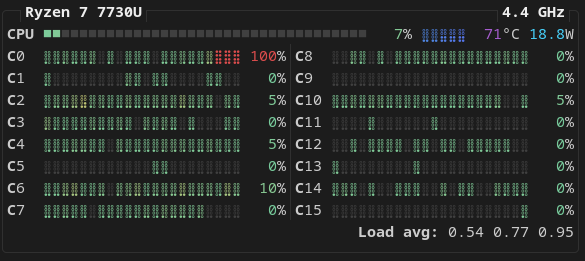
\includegraphics[width=0.8\textwidth]{media/screenshot from 2026-10-12 23-15-04.png}
\caption{Завантаження процесора при дозволеному CPU 0}
\label{fig:cpu-one}
\end{figure}

\begin{figure}[H]
\centering
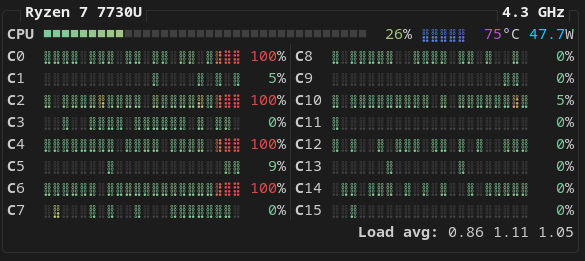
\includegraphics[width=0.8\textwidth]{media/screenshot from 2026-10-12 23-24-19.png}
\caption{Завантаження чотирьох фізичних ядер через CPU 0, 2, 4, 6}
\label{fig:cpu-four}
\end{figure}

\clearpage
\section{Висновки}

У роботі розроблено паралельний алгоритм для виразу варіанта 17.
Обчислення розподілено за елементами векторів і стовпцями проміжної
матриці. Діапазони потоків не перетинаються, тому запис математичних
результатів не потребує взаємного виключення.

Побудовано алгоритми чотирьох потоків із критичними ділянками та
точками синхронізації, а також структурну схему їхньої взаємодії.
М’ютекс усуває перемішування введення й виведення; атомарна операція
об’єднує локальні мінімуми; бар’єри забезпечують готовність даних;
семафор дозволяє $T_1$ дочекатися завершення решти потоків перед друком.

Програму реалізовано мовою C11 з Pthreads. Контрольні тести підтвердили
результати для малих і великих розмірів, від’ємних значень і розмірів,
не кратних чотирьом. Використання \texttt{long long} забезпечило
коректне обчислення для перевірених наборів даних.

За середніми значеннями контрольних запусків прискорення на чотирьох
фізичних ядрах становило $3{,}682$ для $N=1000$ та $3{,}540$ для
$N=1200$. Знімки підтверджують завантаження вибраних CPU. Відхилення
від ідеального прискорення 4 узгоджується з витратами синхронізації,
роботи зі спільною пам’яттю та впливом середовища; окремий внесок цих
чинників у роботі не вимірювався.

\clearpage
\appendix
\section{Лістинг програми}

\subsection{Головний модуль \texttt{main.c}}
\inputminted{c}{../src/main.c}

\subsection{Заголовний файл \texttt{data.h}}
\inputminted{c}{../src/include/data.h}

\subsection{Реалізація модуля \texttt{data.c}}
\inputminted{c}{../src/include/data.c}

\subsection{Файл складання \texttt{CMakeLists.txt}}
\inputminted{cmake}{../src/CMakeLists.txt}

\end{document}
